%%%%%%%%%%%%%%%%%%%%%%%%%%%%%%%%%%%%%%%%%
% Beamer Presentation
% LaTeX Template
% Version 1.0 (10/11/12)
%
% This template has been downloaded from:
% http://www.LaTeXTemplates.com
%
% License:
% CC BY-NC-SA 3.0 (http://creativecommons.org/licenses/by-nc-sa/3.0/)
%
%%%%%%%%%%%%%%%%%%%%%%%%%%%%%%%%%%%%%%%%%

%----------------------------------------------------------------------------------------
%	PACKAGES AND THEMES
%----------------------------------------------------------------------------------------

\documentclass[xcolor=table]{beamer}

\mode<presentation> {

% The Beamer class comes with a number of default slide themes
% which change the colors and layouts of slides. Below this is a list
% of all the themes, uncomment each in turn to see what they look like.

%\usetheme{default}
%\usetheme{AnnArbor}
%\usetheme{Antibes}
%\usetheme{Bergen}
\usetheme{Berkeley}
%\usetheme{Berlin}
%\usetheme{Boadilla}
%\usetheme{CambridgeUS}
%\usetheme{Copenhagen}
%\usetheme{Darmstadt}
%\usetheme{Dresden}
%\usetheme{Frankfurt}
%\usetheme{Goettingen}
%\usetheme{Hannover}
%\usetheme{Ilmenau}
%\usetheme{JuanLesPins}
%\usetheme{Luebeck}
%\usetheme{Madrid}
%\usetheme{Malmoe}
%\usetheme{Marburg}
%\usetheme{Montpellier}
%\usetheme{PaloAlto}
%\usetheme{Pittsburgh}
%\usetheme{Rochester}
%\usetheme{Singapore}
%\usetheme{Szeged}
%\usetheme{Warsaw}

% As well as themes, the Beamer class has a number of color themes
% for any slide theme. Uncomment each of these in turn to see how it
% changes the colors of your current slide theme.

%\usecolortheme{albatross}
%\usecolortheme{beaver}
%\usecolortheme{beetle}
%\usecolortheme{crane}
%\usecolortheme{dolphin}
%\usecolortheme{dove}
%\usecolortheme{fly}
%\usecolortheme{lily}
%\usecolortheme{orchid}
%\usecolortheme{rose}
%\usecolortheme{seagull}
%\usecolortheme{seahorse}
%\usecolortheme{whale}
%\usecolortheme{wolverine}
%\setbeamertemplate{footline} % To remove the footer line in all slides uncomment this line
\setbeamertemplate{footline}[page number] % To replace the footer line in all slides with a simple slide count uncomment this line

\setbeamertemplate{navigation symbols}{} % To remove the navigation symbols from the bottom of all slides uncomment this line 
}
\usepackage{amsmath} 
\usepackage{graphicx} % Allows including images
\usepackage{booktabs} % Allows the use of \toprule, \midrule and \bottomrule in tables
\usepackage[table]{xcolor}

%\usepackage[style=ieee]{biblatex} %Use if necessary for citation
%\addbibresource{biblatex-examples.bib}
%----------------------------------------------------------------------------------------
%	TITLE PAGE
%----------------------------------------------------------------------------------------

\title[PPI Graphs]{Protein-Protein Interaction Graph} % The short title appears at the bottom of every slide, the full title is only on the title page

\author{Nathanael Roy} % Your name
\institute[UCR] % Your institution as it will appear on the bottom of every slide, may be shorthand to save space
{
University of California, Riverside \\ % Your institution for the title page
\medskip
}
\date{\today} % Date, can be changed to a custom date

\begin{document}

\begin{frame}
\titlepage % Print the title page as the first slide
\end{frame}

\begin{frame}{Reading in Data}
    \begin{itemize}
        \item Read in Edge List http text file as a table
        \item Treat Each Protein as the number it is associated with
        \item Use Regular Expression format in R to parse the table and to shift into more acceptable format
        \item Use package "igraph" to save as a graph object in package
    \end{itemize}
\end{frame}

\begin{frame}{Some Basic Information}
\begin{itemize}
    \item Connected: Whether we can traverse the graph
    \item Number of disconnected subgraphs of each PPI graph, how many "sub families" of proteins: It turns out most proteins can be grouped together although the graph is disconnected
    \item Number of edges and vertices in the graph, how many interactions and how many proteins
    \item Average degree of vertices, how many neighbors represents immediate interactions
\end{itemize}
\end{frame}

\begin{frame}{Some Centrality Information}
\begin{itemize}
    \item Diameter: The longest path for two connected vertices. This gives an idea that if there is a complex interaction between proteins it is at most this far away. This is also defined as maximum eccentricity
    \item Degree Centrality: An intuitive way of understanding this is as a fraction of how close the graph is to a star graph. The Degree Centrality of a graph is calculated as $\frac{\sum_{\forall i} deg(v*)-deg(v_i))}{H}$ where $v*$ has highest degree,  $H$ is the value in the numerator for a star graph: $(n^2-3n+2)$
    \item Betweenness: Number of shortest paths that pass through a vertex
    \item Clustering Coefficient: How close the neighbors of a vertex are to being a complete graph $K_n$
\end{itemize}
\end{frame}

\begin{frame}{Measures for Fly and Yeast PPI Graphs}
    \begin{table}[H]
\begin{center}
\begin{tabular}{ |c|c|c|  }

\hline
\multicolumn{3}{|c|}{Fly and Yeast Graph} \\
\hline
\rowcolor{gray!50}
Value & Fly Graph &Yeast Graph \\
\hline
Connected &No &No\\
Disconnected Parts & 73 & 44 \\
Number of Edges &20988 & 15466\\
Number of Vertices & 7068 & 4773\\
Average Degree & 5.9389   & 6.4785 \\
Diameter (longest path) & 11 & 12 \\
Diameter for Directed Graph & 15&17 \\
Clustering Coefficient  & .01170 & .05942 \\
Degree Centrality (Directed) & .01218 &  .02898 \\
Degree Centrality (Undirected) & .02435 &  .05795 \\

Betweenness (Directed)&  1294.786 & 8193.767   \\
Betweenness (Undirected)&  11737.22 & 7328.424   \\

\hline
\end{tabular}
\end{center}
\end{table}
\end{frame}

\begin{frame}{Some Initial Observations}
    \begin{itemize}
        \item Neither graph is connected but does have a distinct subgraph that is connected and contains the vast majority of proteins and connections
        \item The longest diameters are relatively short despite the large number of vertices and relatively small average degree
        \item Both degree centrality and clustering coefficient are small, neither graph is close to a star graph nor to a complete graph
        \item There are over 24 million possible paths for the fly graph (7068 choose 2) and over 11 million for the yeast graph. At first glance it seems like the average betweenness is high for both but it seems to not be the case
    \end{itemize}
\end{frame}

\begin{frame}{Longest Path: Fly (Directed)}
\begin{figure}[H]
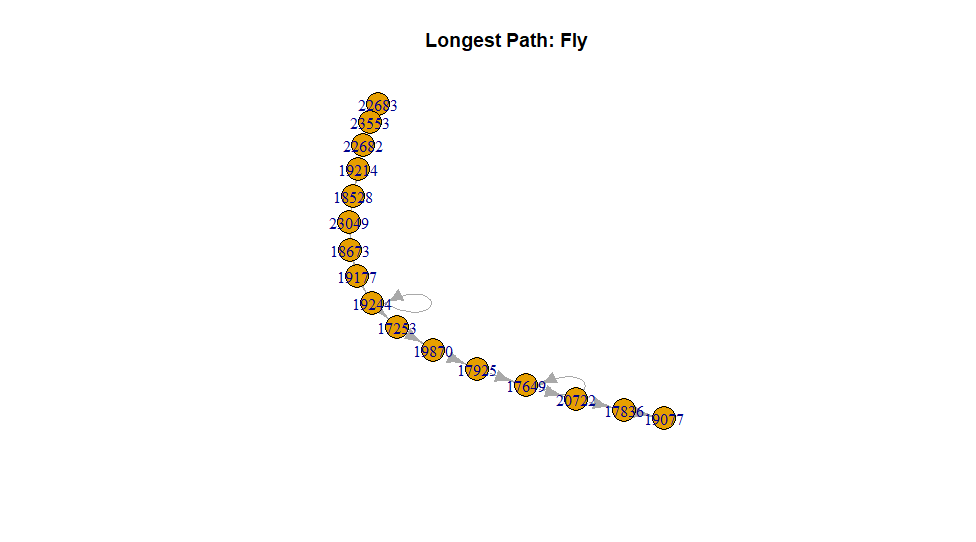
\includegraphics[width=\linewidth]{LPFly.png}
\end{figure}
\end{frame}

\begin{frame}{Longest Path: Yeast (Directed)}
    \begin{figure}[H]
\centering
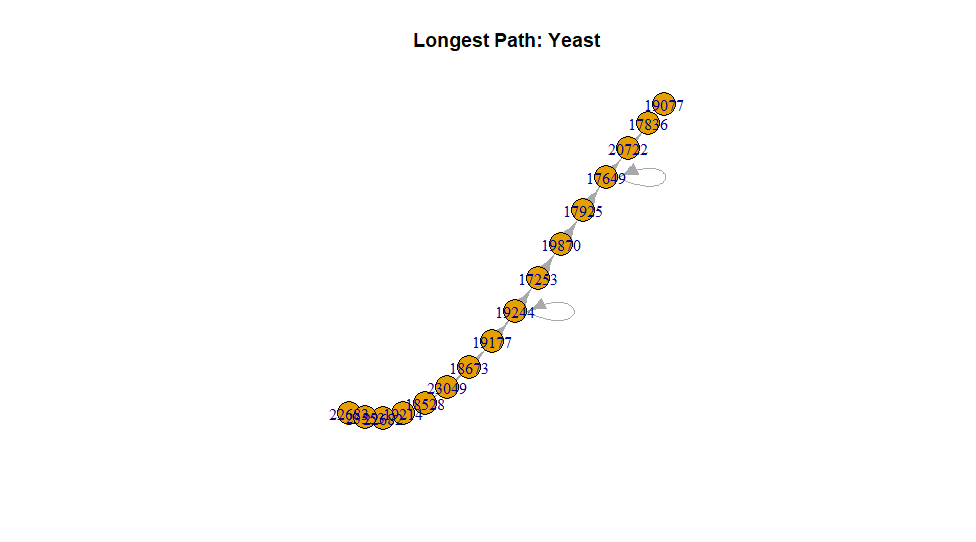
\includegraphics[width=\linewidth]{LPYeast.png}
\end{figure}
\end{frame}
\begin{frame}{Scale Free Distribution}
    \begin{itemize}
        \item The next couple o graphs give the distribution of degrees of vertices
        \item Plotted on a log scale: Should be linear assuming scale-free property of graph holds
        \item Yeast doesn't seem to follow the scale free property as closelyas the fly PPI graph does, or at least the histogram may not be the best visualization
    \end{itemize}
\end{frame}
\begin{frame}{Degree Distribution: Fly}
    \begin{figure}[H]
\centering
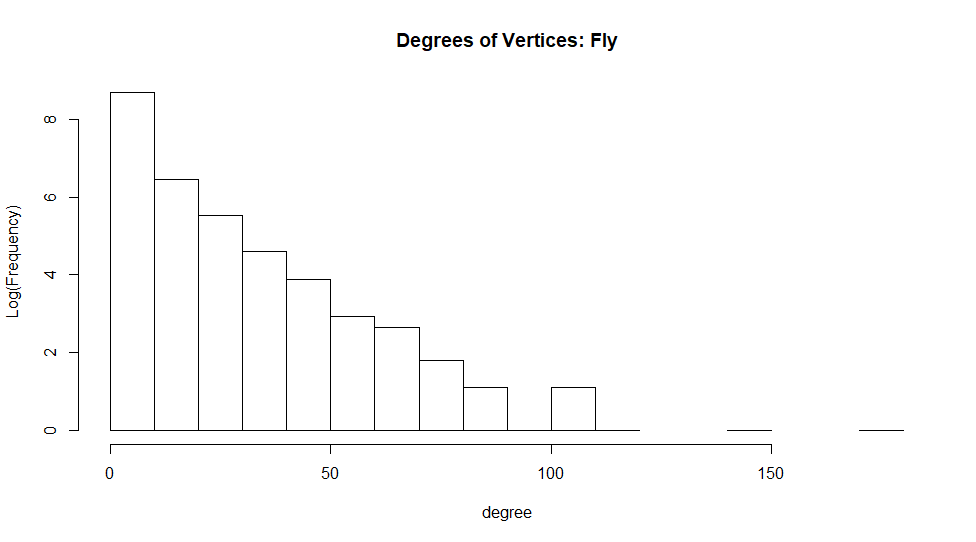
\includegraphics[width=\linewidth]{DegVFly.png}
\end{figure}
\end{frame}

\begin{frame}{Degree Distribution: Yeast}
    \begin{figure}[H]
\centering
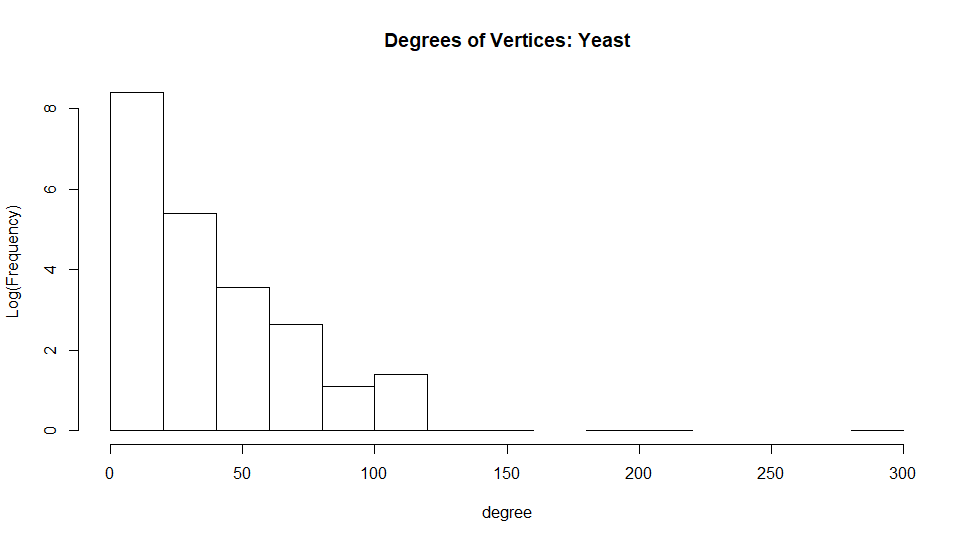
\includegraphics[width=\linewidth]{DegVYeast.png}
\end{figure}
\end{frame}

\begin{frame}{Betweenness Graphs: A Few Proteins Dominate}
    \begin{itemize}
        \item For our Fly graph it seems that there are two "clusters" of proteins by name.
        \item Seems to be an exponential decay as the protein number increases once we reach a present protein
        \item A few proteins seem more dominant in terms of betweenness
        \item Yeast follows a similar pattern but it is less clear, once again though a few proteins have a great deal more betweenness than other proteins
    \end{itemize}
\end{frame}
\begin{frame}{Betweenness: Fly}
    \begin{figure}[H]
\centering
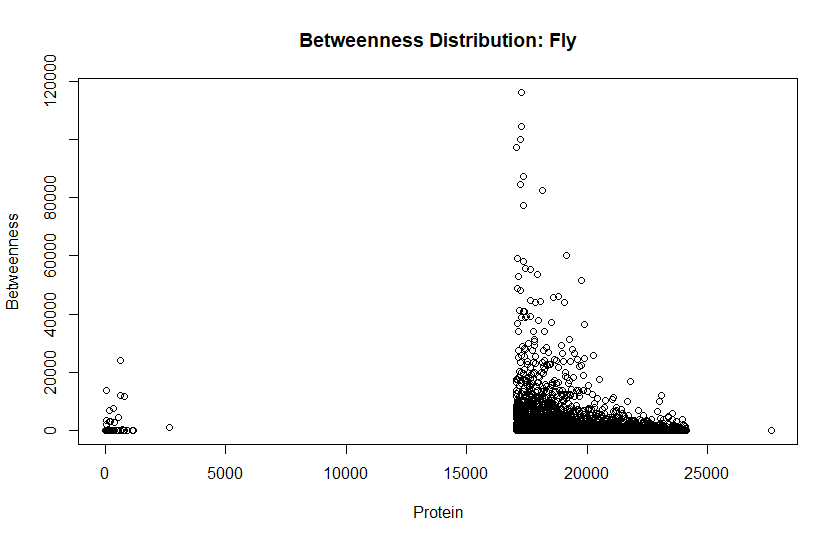
\includegraphics[width=\linewidth]{BetweenFly.png}
\end{figure}
\end{frame}

\begin{frame}{Betweenness: Yeast}
    \begin{figure}[H]
\centering
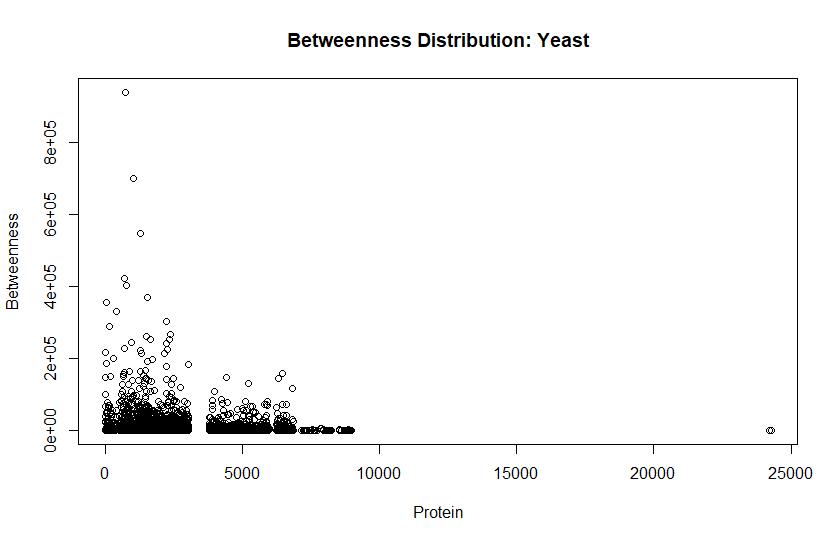
\includegraphics[width=\linewidth]{BetweenYeast.png}
\end{figure}
\end{frame}

\begin{frame}{Eccentricity}
    Eccentricity seems to be 7 for most of the vertices in the graphs for both Fly and Yeast and the distribution of eccentricity is very similar between the two networks. The similarities between the two graphs on this trait is actually fairly striking to me. Most proteins are just about 7 interactions away from any other vertex at most.
    
    Particularly striking: The radius of the connected graph with most of the vertices is 6 for both graphs
\end{frame}

\begin{frame}{Eccentricity Distribution: Fly}
\begin{figure}[H]
\centering
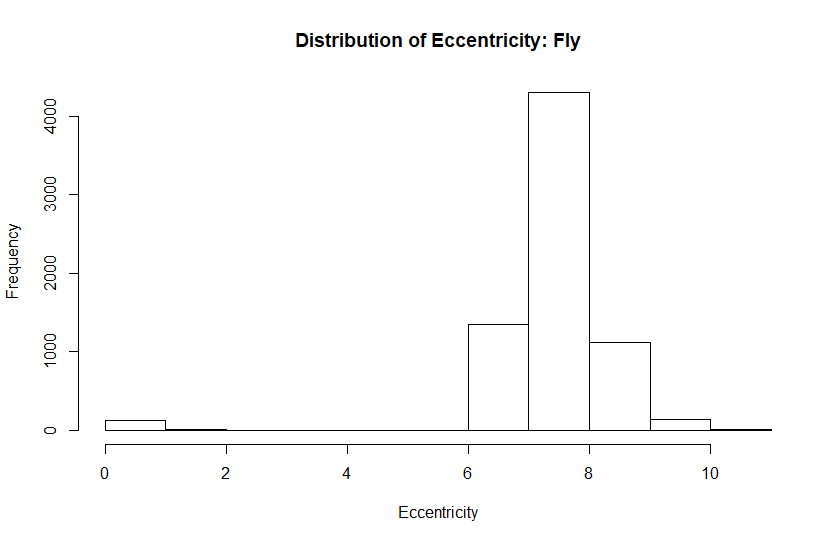
\includegraphics[width=\linewidth]{EccentricityFly.png}
\end{figure}
\end{frame}


\begin{frame}{Eccentricity Distribution: Yeast}
\begin{figure}[H]
\centering
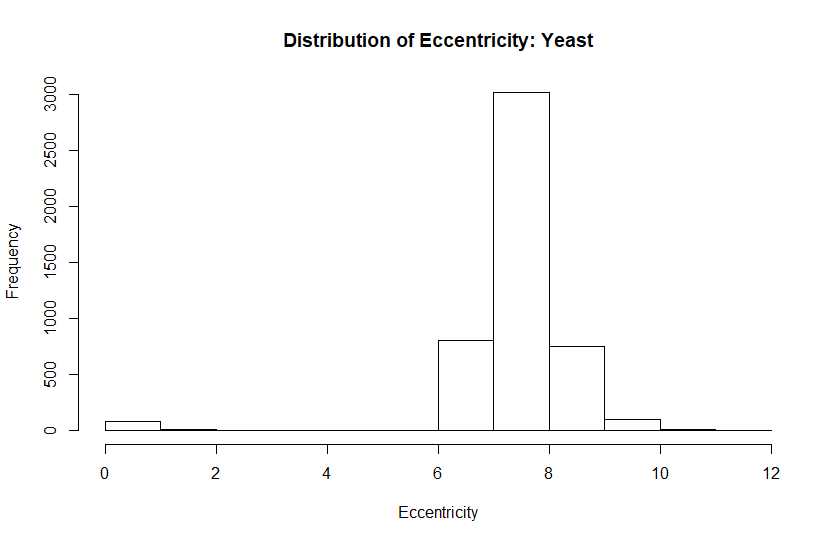
\includegraphics[width=\linewidth]{EccentricityYeast.png}
\end{figure}
\end{frame}

\begin{frame}{Discussion; Future Consideration}
    \begin{itemize}
        \item Ran out of time to create an R shiny app; could have made such an app to be able to plot subgraphs in a user friendly way
        \item connectivity questions 
        \item Since we can view the edges as directed, perhaps I could try to find chain pairs and ultrabubles. 
        
    \end{itemize}
\end{frame}
\end{document}